\documentclass{article}

% NeurIPS 2026 double-blind workshop submission.
\usepackage[dblblindworkshop]{neurips_2026}
\workshoptitle{Physical World AI: Geometry, Characteristics, and Multimodal Sensing}

\usepackage[utf8]{inputenc}
\usepackage[T1]{fontenc}
\usepackage{hyperref}
\usepackage{url}
\usepackage{booktabs}
\usepackage{amsfonts}
\usepackage{amsmath}
\usepackage{amssymb}
\usepackage{nicefrac}
\usepackage{microtype}
\usepackage{graphicx}
\usepackage{xcolor}

\graphicspath{{figures/}}

\title{Build the Geometry In, Don't Hope It Emerges:\\ A Reflection-Symmetry Audit of a Skeleton World Model}

% Anonymous for double-blind review (the [dblblindworkshop] option renders
% "Anonymous Author(s)" and suppresses the affiliation block).
\author{%
  Anonymous Author(s)\\
  Affiliation\\
  Address\\
  \texttt{email}\\
}

\begin{document}

\maketitle

\begin{abstract}
Bilateral (left--right) reflection is the most basic geometric symmetry of the articulated human body: mirroring a skeleton across the sagittal plane and swapping left/right landmarks yields another valid skeleton, so the operation generates a $\mathbb{Z}/2$ group acting on skeleton space. We ask whether a self-supervised skeleton world model---a masked-latent-infilling S-JEPA over 33-joint pose sequences---encodes this symmetry as a decodable, sign-flipping \emph{laterality} axis. We turn the question into an exact group-action equivariance test: a signed left-minus-right motion target that is antisymmetric under the mirror by construction ($y(Mx)=-y(x)$), probed under source-video-disjoint, repeated cross-validation against a raw-coordinate ceiling, an untrained-encoder floor, a side-blind pooled control, and a landmark-missingness control. On the frozen curriculum encoder the answer is a \textbf{robust informative null}: the learned laterality feature reaches only $R^2=0.198$ (stability interval $[0.175,0.221]$)---below the untrained floor in repeated-CV mean ($0.245$ $[0.214,0.275]$; the stability intervals overlap, a partition-stability heuristic rather than a significance test)---with a mirror slope of $-0.70$ instead of the required $-1$; all three pre-registered gates fail. We then show the geometry can be \textbf{recovered by construction}: a frame-averaged read-out over $\{I,M\}$ is exactly antisymmetric (mirror slope $-1.0000$ for any nonzero weights) and reaches $R^2=0.273$ $[0.253,0.294]$, above the free read-out in repeated-CV mean with disjoint stability intervals (again a stability heuristic, not a formal test); a frame-averaged \emph{encoder} wrapper is exactly token-equivariant with zero retraining (equivariance error $0.0$). Finally, in a single-seed ablation, reflection \emph{augmentation} during pretraining does \textbf{not} induce the property (augmented axis $0.062$, not clearing floor $0.078$; slope no closer to $-1$). The lesson is a design principle for geometry-aware world models of articulated bodies: \emph{build the symmetry in; do not hope it emerges.} All results are transductive (internal validity only); the source video is the independent unit; dataset folder labels are annotations, not diagnoses.
\end{abstract}

\section{Introduction}

Physical-world scene understanding increasingly relies on \emph{world models}---self-supervised predictors that learn latent dynamics without labels. For articulated bodies, a natural question is whether such models internalize the body's \textbf{geometry}. The most elementary geometric fact about a human skeleton is bilateral symmetry: reflecting it across the sagittal plane and relabeling left as right produces a physically valid skeleton. This is not a nuisance transformation to be averaged away; it is a \emph{structural prior} that a competent world model of an articulated body might be expected to respect.

We study whether a frozen skeleton world model---an S-JEPA encoder trained by masked latent infilling over 33-joint BlazePose \citep{grishchenko2022blazepose, mediapipePoseLandmarker} sequences---has learned bilateral symmetry in a form that is \emph{decodable} and \emph{sign-correct}. We make the question exact by treating the mirror as a group action. The mirror operator $M$ (negate $x$; swap all sixteen bilateral left/right landmark pairs---a valid whole-body reflection) satisfies $M^2=I$, so $\{I,M\}\cong\mathbb{Z}/2$. We define a scalar \textbf{signed laterality} target measuring which side of the body moves more; by construction it is antisymmetric, $y(Mx)=-y(x)$. The world model ``knows'' bilateral symmetry iff its decoded laterality flips sign when the input is mirrored---a linear mirror slope of $-1$---while remaining decodable at all (Fig.~\ref{fig:group}).

\begin{figure}[t]
  \centering
  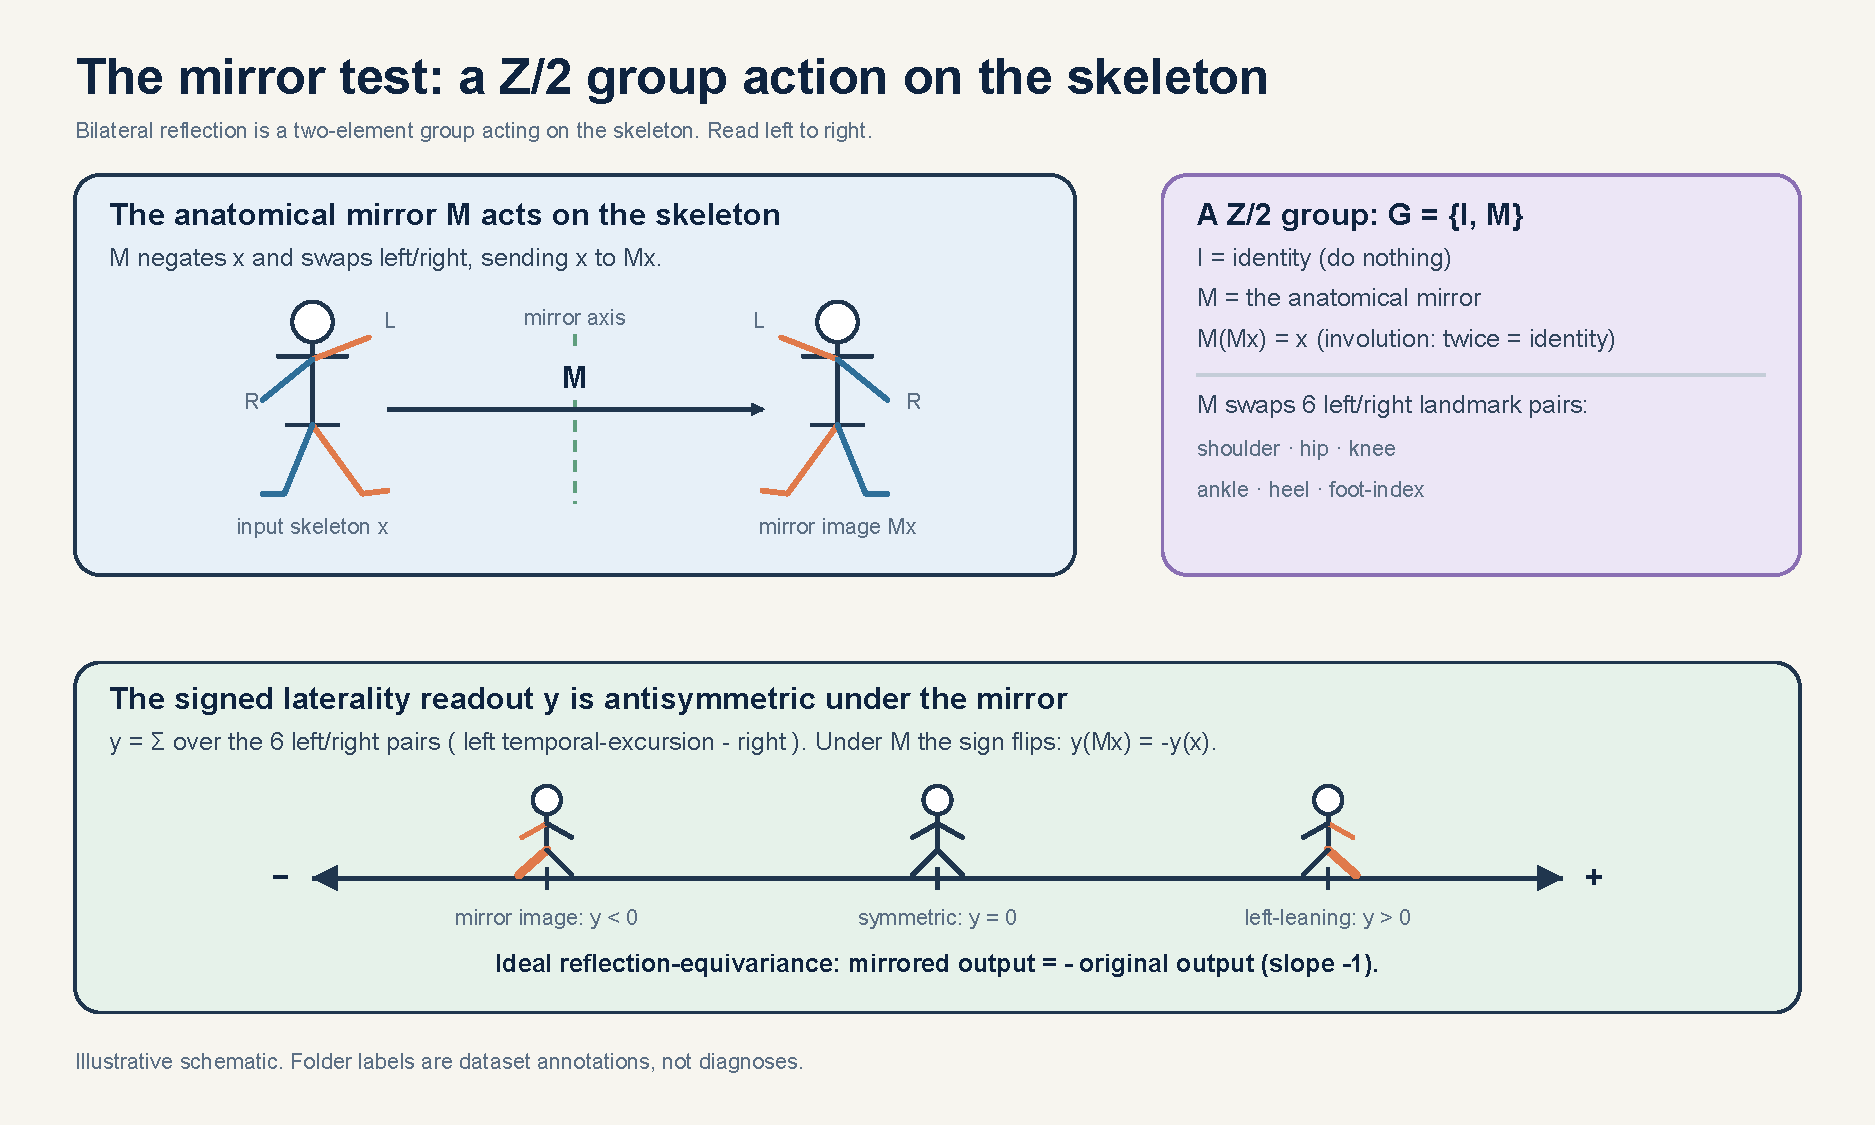
\includegraphics[width=0.62\linewidth]{fig1_group_action.pdf}
  \caption{Bilateral reflection as a $\mathbb{Z}/2$ group action. The mirror $M$ negates the sagittal coordinate and swaps left/right landmarks; the signed laterality target is antisymmetric by construction, $y(Mx)=-y(x)$, so ``encoding the symmetry'' means a decoded mirror slope of exactly $-1$.}
  \label{fig:group}
\end{figure}

\paragraph{Contributions.}
\begin{enumerate}
\item \textbf{A reusable geometry audit} for skeleton world models: an exact $\mathbb{Z}/2$ mirror test with a raw ceiling, an untrained floor, a side-blind control, and a missingness control, evaluated under source-disjoint \emph{repeated} cross-validation with pre-registered gates (Fig.~\ref{fig:audit}).
\item \textbf{An informative null with uncertainty.} The audited curriculum checkpoint \emph{fails} the audit: the learned laterality feature does not beat the untrained floor under repeated CV, and the mirror slope is $-0.70$, not $-1$ (\S\ref{sec:e1}, Fig.~\ref{fig:null}). We characterize the failure---an alpha-sensitivity sweep shows the feature is decodable only under heavy regularization, consistent with (but not proving) a weak, collinear geometry.
\item \textbf{A constructive fix by group averaging.} A frame-averaged read-out is antisymmetric by construction (slope $-1.0000$) and beats the free read-out in repeated-CV mean with disjoint stability intervals (a partition-stability heuristic); a frame-averaged encoder is exactly token-equivariant with zero retraining (\S\ref{sec:e2}--\S\ref{sec:e3}, Figs.~\ref{fig:construction}--\ref{fig:builtin}).
\item \textbf{A negative result for augmentation.} In the audited single-seed Stage-0 arm, reflection augmentation during pretraining did not induce the symmetry (\S\ref{sec:e32}), sharpening the design principle: \emph{build it in, do not hope it emerges} (Fig.~\ref{fig:ladder}).
\end{enumerate}

We connect throughout to the workshop's themes: this is a \textbf{geometry-aware} probe (and fix) of a world model for an \textbf{articulated, deformable} body, whose target is a \textbf{proprioceptive} quantity---which side moves more.

\section{Related work}

\paragraph{Equivariant and geometric deep learning.} Group-equivariant networks build symmetry into the architecture, from group-convolutions and steerable CNNs \citep{cohen2016gcnn, cohen2017steerable, weiler2019e2cnn, weiler2018steerable3d, worrall2017harmonic} to equivariant graph and attention networks \citep{satorras2021egnn, fuchs2020se3}, unified under the geometric-deep-learning program \citep{bronstein2021gdl}. Rather than constrain every layer, \emph{frame averaging} attains exact equivariance by symmetrizing over a group (or a frame of it) around an arbitrary backbone \citep{puny2022frame}, and \emph{canonicalization} learns to align inputs to a canonical pose \citep{kaba2023canonicalization, jaderberg2015stn}. A complementary line asks whether symmetry can instead be \emph{learned from data} via augmentation \citep{benton2020augerino}. Our read-out and encoder constructions are frame averaging over $\mathbb{Z}/2$; our augmentation arm is a direct test of the learned-invariance hypothesis.

\paragraph{Self-supervised skeleton models.} Skeleton action recognition is dominated by spatio-temporal graph networks \citep{yan2018stgcn, shi2019agcn}; recent self-supervised approaches use masked prediction and joint-embedding objectives \citep{abdelfattah2024sjepa, mao2023mamp, xu2024skeleton2vec}, echoing image/video JEPA \citep{assran2023ijepa, bardes2024vjepa} and VICReg-style regularization \citep{bardes2022vicreg}. These works optimize for downstream accuracy; none audit whether the learned latent respects the body's reflection symmetry as an exact, sign-flipping axis.

\paragraph{Gait symmetry.} Clinically, left--right symmetry indices are established descriptors of healthy and pathological gait \citep{sadeghi2000symmetry, patterson2010symmetry, robinson1987symmetry, blazkiewicz2014symmetry}. We borrow the \emph{concept} of a signed bilateral asymmetry but use it purely as a geometric decodability target on public pose data---not as a clinical measurement.

\section{Bilateral symmetry as a group action}

\paragraph{Group and operator.} Let $x\in\mathbb{R}^{T\times 33\times 3}$ be a pose sequence. The mirror $M$ negates the $x$-coordinate of every joint and applies the left/right permutation that swaps all sixteen bilateral BlazePose landmark pairs---a valid whole-body reflection. Then $M^2=I$ and $G=\{I,M\}\cong\mathbb{Z}/2$.

\paragraph{Target.} For each of the six bilateral pairs $(11,12),(23,24),(25,26),(27,28),(29,30),(31,32)$ (shoulders, hips, knees, ankles, heels, foot-indices), let $\ell_k$ (resp.\ $r_k$) be the per-joint temporal standard deviation of the left (resp.\ right) landmark summed over $x,y,z$. The signed laterality target is $y(x)=\sum_k(\ell_k-r_k)$. Mirroring swaps $\ell_k\leftrightarrow r_k$, so
\[ y(Mx) = -\,y(x). \]
This is a group-action equivariance condition $y(T_g\,x)=\rho(g)\,y(x)$ with the sign representation $\rho(I)=+1,\ \rho(M)=-1$. A model ``encodes bilateral symmetry'' iff a read-out of its features reproduces this antisymmetry: \textbf{mirror slope $-1$}, while being decodable ($R^2$ well above floor).

\paragraph{Backbone.} The world model is a frozen S-JEPA (config: 64 frames, 33 joints, segment length 4, embed dim 96, 4-layer encoder, 2-layer predictor, 4 heads; masked latent infilling with a VICReg term), trained by a curriculum beginning with the \texttt{normal}-annotated rows and adding each annotated condition. We bind all results to a single checkpoint (fingerprint \texttt{7d13841a\ldots}). The primary cohort is the \textbf{626} sequences / \textbf{93} source videos the encoder actually trained on (fully transductive); a \textbf{642}/94 superset is reported only for robustness.

\section{The audit protocol}\label{sec:audit}

\begin{figure}[t]
  \centering
  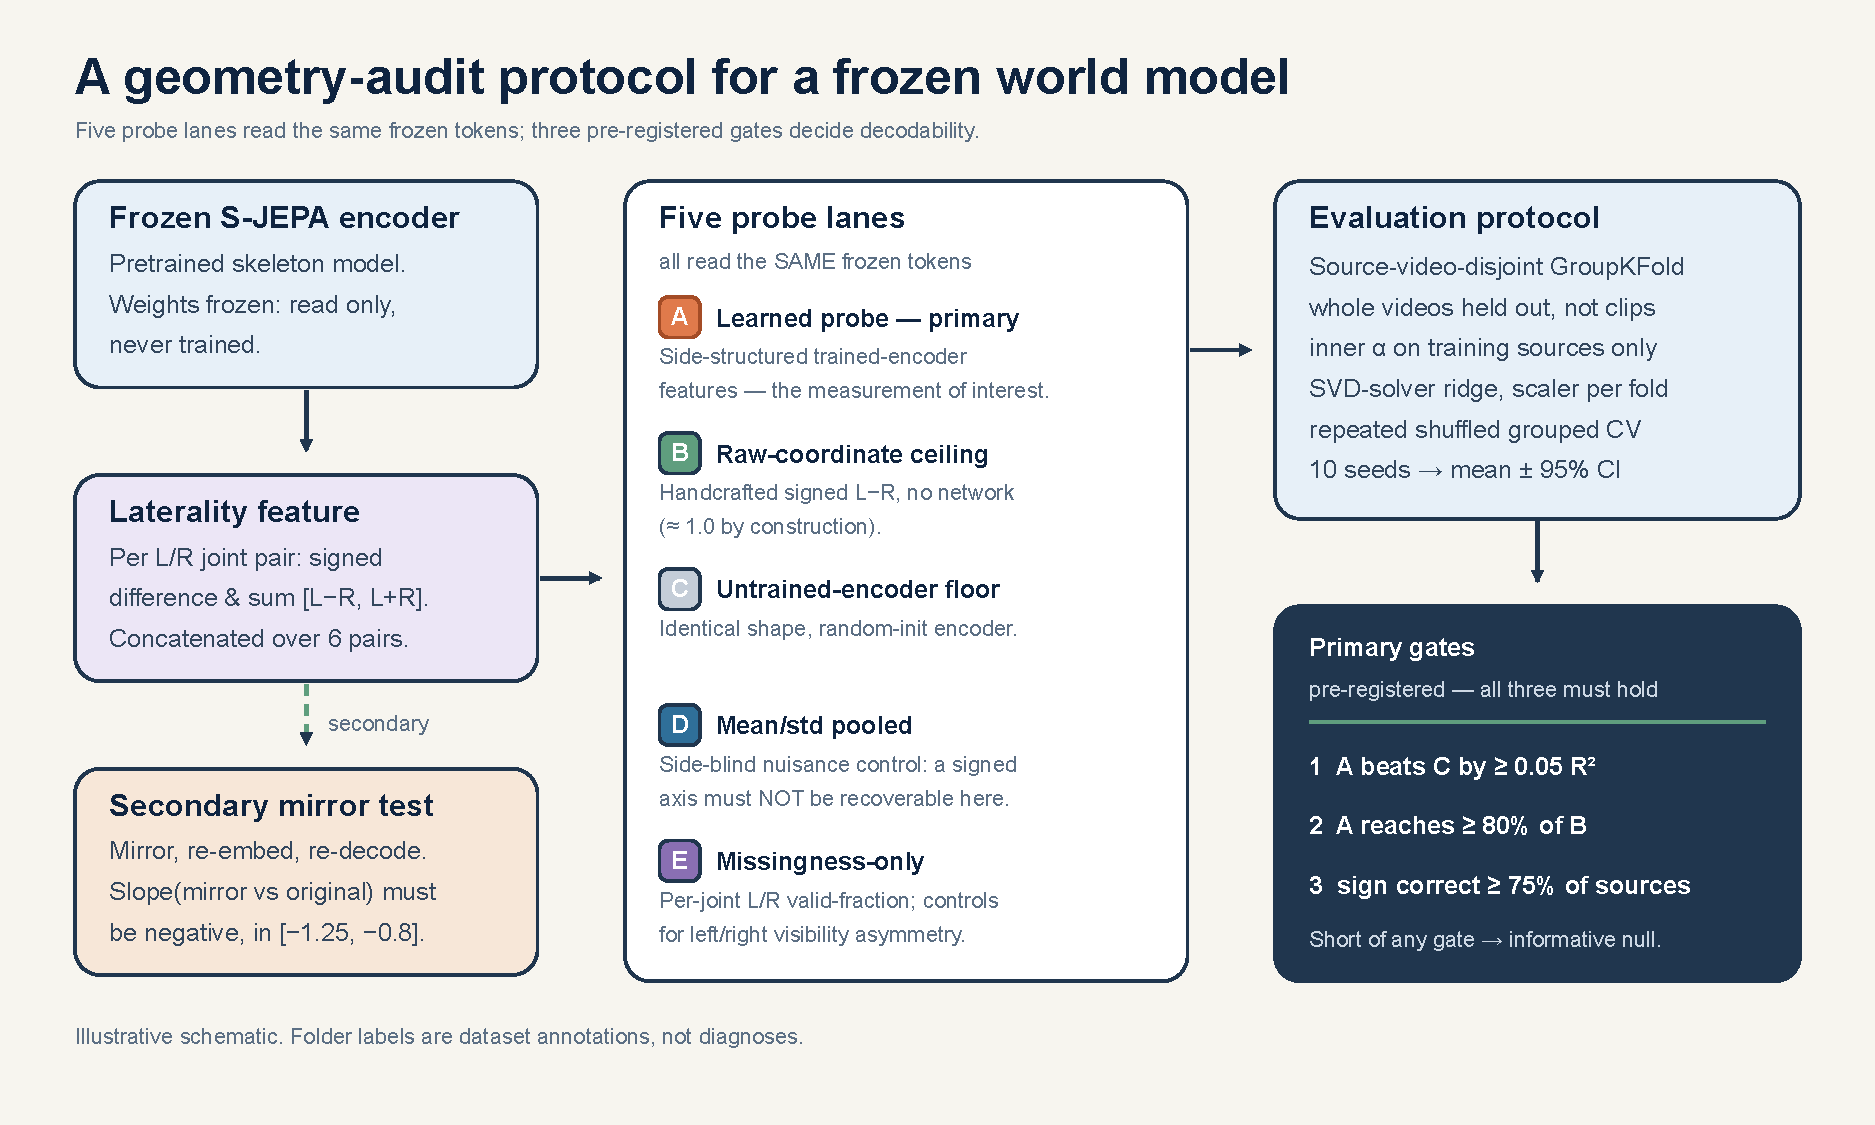
\includegraphics[width=0.74\linewidth]{fig2_audit_protocol.pdf}
  \caption{The five-lane audit. A learned per-pair token statistics; B raw-coordinate ceiling ($R^2\approx1$); C untrained-encoder floor; D side-blind pooled control; E landmark-missingness control. Estimation is source-video-disjoint \texttt{GroupKFold} repeated over ten reshuffles of a fixed cohort, with pre-registered gates.}
  \label{fig:audit}
\end{figure}

\paragraph{Five lanes} (Fig.~\ref{fig:audit}). \textbf{A --- learned}: per-pair $[\ell-r,\ \ell+r]$ token statistics from the frozen encoder. \textbf{B --- raw ceiling}: target from coordinates ($R^2\approx1$), a decodability sanity check. \textbf{C --- floor}: identical architecture, random weights. \textbf{D --- pooled}: whole-body mean/std, side-blind (must stay low). \textbf{E --- missingness}: per-joint left/right valid-fraction (must stay low; if it rivals A, the learned score may reflect left/right visibility asymmetry rather than motion).

\paragraph{Estimator.} Source-disjoint \texttt{GroupKFold}; inner ridge-penalty selection over $\alpha\in\mathrm{logspace}(-3,3,13)$; per-fold standardization; SVD solver (used to reduce sensitivity to the numerical ill-conditioning seen in the original run). We repeat the whole grouped CV over 10 reshuffles of the \emph{fixed} 626-sequence / 93-source cohort and report the mean with a $t$-based interval ($\mathrm{df}=9$, $t^*=2.262$). Because every reshuffle re-partitions the same fixed rows, this is an \textbf{across-reshuffle stability interval}: it quantifies sensitivity to the CV partition, not sampling variability over a population, and carries no out-of-sample or generalization guarantee \citep{bengio2004variance, roberts2017crossvalidation}. Interval overlap or non-overlap is therefore a stability heuristic, not a formal significance test.

\paragraph{Pre-registered gates.} (i)~A beats C by $\ge 0.05$ $R^2$; (ii)~A reaches $\ge 80\%$ of B; (iii)~sign correct on $\ge 75\%$ of held-out sources. \textbf{Secondary geometry band:} mirror slope negative and within $[-1.25,-0.80]$.

\section{E1 --- the emergent null, hardened}\label{sec:e1}

Table~\ref{tab:e1} reports the five lanes on the primary cohort.

\begin{table}[t]
  \centering
  \caption{E1 laterality probe (626 primary, canonical checkpoint).}
  \label{tab:e1}
  \begin{tabular}{lrr}
    \toprule
    Lane & Single-partition $R^2$ & Repeated-CV $R^2$ (stability interval) \\
    \midrule
    A --- learned            & 0.268    & \textbf{0.198 [0.175, 0.221]} \\
    C --- untrained floor    & 0.229    & \textbf{0.245 [0.214, 0.275]} \\
    D --- pooled (side-blind)& 0.107    & 0.101 [0.089, 0.114] \\
    E --- missingness-only   & 0.162    & 0.202 [0.173, 0.231] \\
    B --- raw ceiling        & $\approx$1.000 & --- \\
    \bottomrule
  \end{tabular}
\end{table}

\begin{figure}[t]
  \centering
  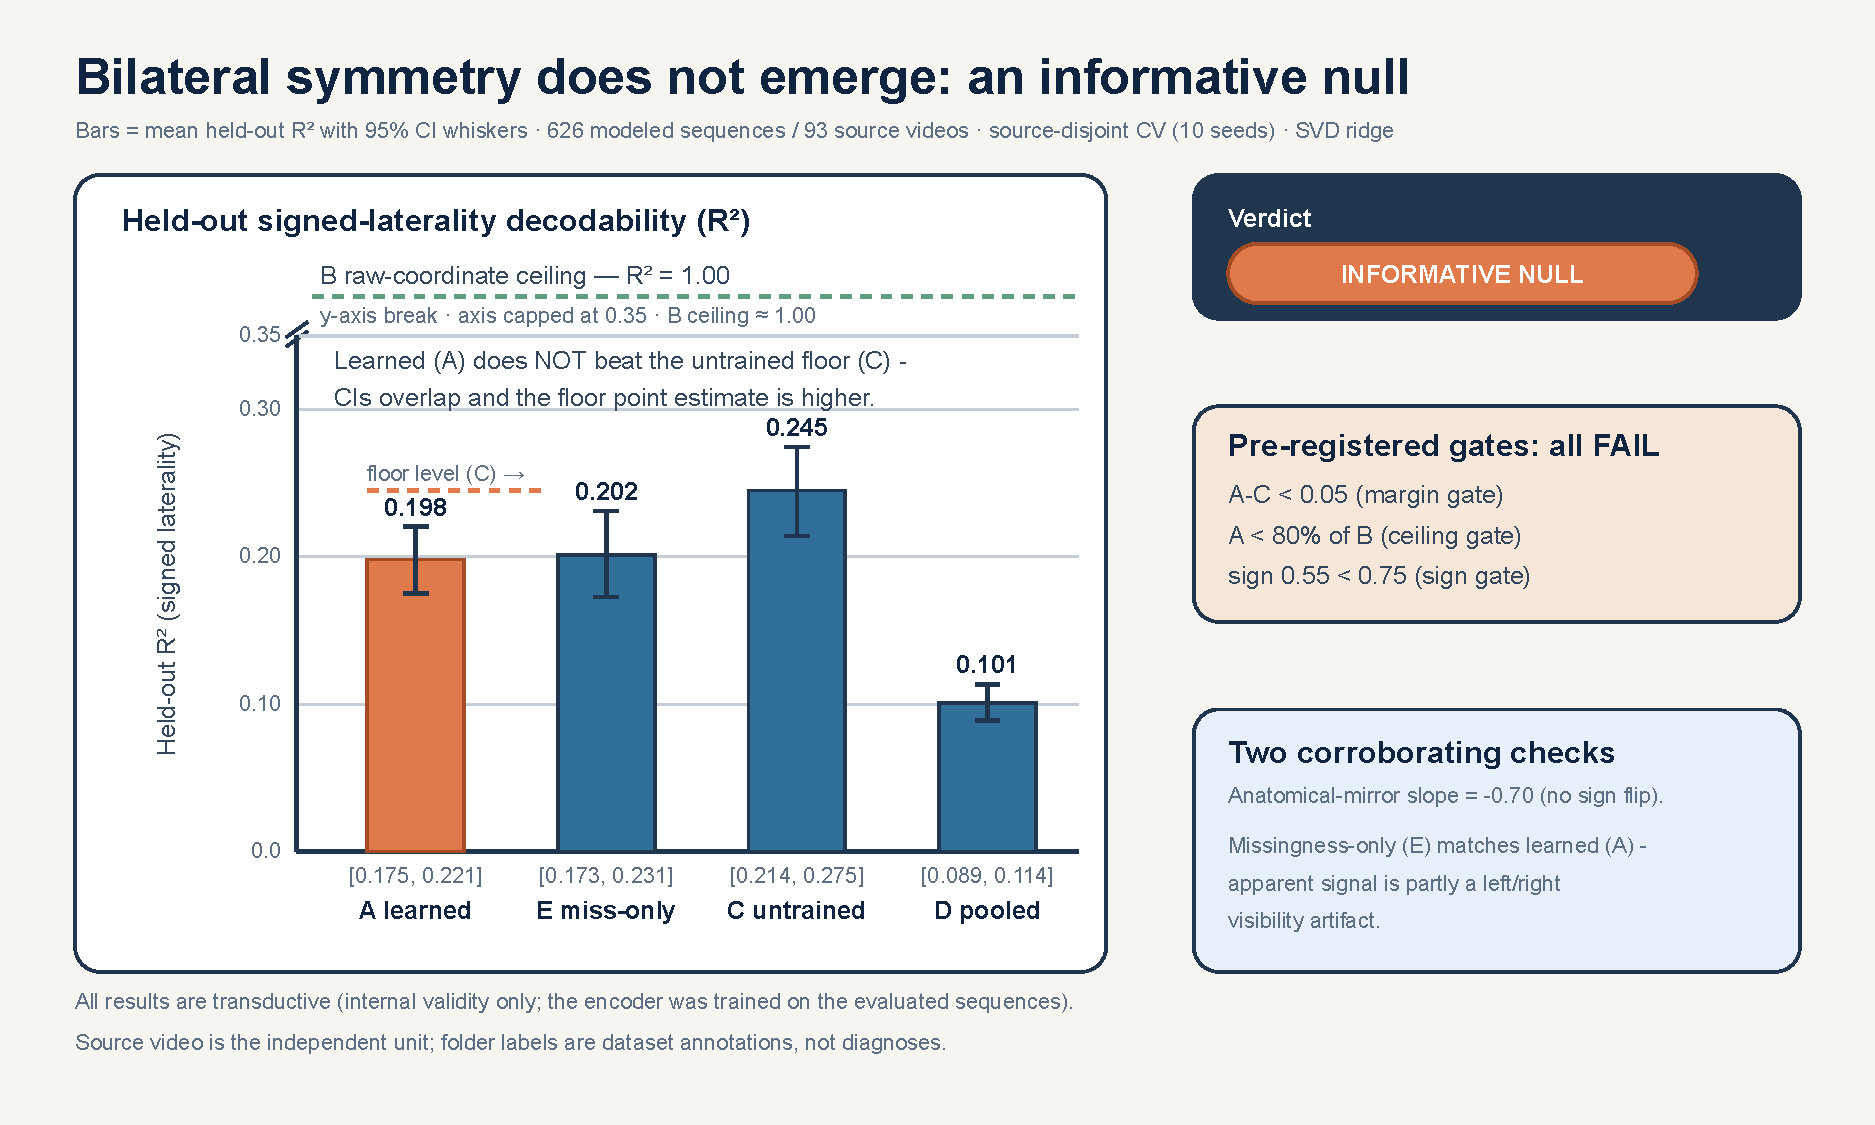
\includegraphics[width=0.74\linewidth]{fig3_e1_null.pdf}
  \caption{The hardened null. Under repeated CV the learned lane A sits below the untrained floor C in mean with overlapping stability intervals; the single-partition ordering $A>C$ reverses. The alpha sweep rises monotonically from $-2.04$ to $+0.268$, decodable only under heavy regularization---consistent with a weak, collinear feature.}
  \label{fig:null}
\end{figure}

Mirror slope $-0.703$ (no sign flip); sign consistency $0.576$ $[0.548,0.604]$. \textbf{All three gates fail.} The decisive observation is that the single-partition ordering $A(0.268)>C(0.229)$ \emph{reverses} under repeated CV, $A(0.198)<C(0.245)$: the original notebook's lone ``win'' was a single partition near the top of A's spread (maximum across the ten CV reshuffles $0.272$). An alpha sweep shows A's score rising monotonically from $-2.04$ at $\alpha=10^{-3}$ to $+0.268$ at $\alpha\ge316$---a feature decodable only under heavy regularization is consistent with a weak, collinear geometry, not a clean axis (Fig.~\ref{fig:null}). The 642 robustness cohort reproduces the pre-hardening numbers bit-for-bit ($A=0.241$, $C=0.190$, slope $-0.627$) and is the \emph{only} configuration where gate (i) passes on a single partition; it does not survive cohort-matching plus repeated CV. The missingness control behaves consistently with the null: under repeated CV, Lane E ($0.202$ $[0.173,0.231]$) has a repeated-CV mean close to learned Lane A ($0.198$), which flags possible visibility confounding rather than establishing equivalence---corroborating, not undermining, the null. (The single-partition \texttt{missingness\_control\_ok} flag, on which E sits below A, does not survive repeated CV, and E is itself estimator- and cohort-sensitive---$0.162$ single vs $0.202$ repeated on 626, and $0.047$ on the 642 superset---so we read it only as corroboration.) \textbf{Verdict: a robust informative null}---the world model did not learn bilateral symmetry as a decodable, sign-flipping axis.

\section{E2 --- reflection-equivariant read-out by construction}\label{sec:e2}

Rather than hope the frozen feature $A(x)$ is antisymmetric, we \textbf{average over the group} \citep{puny2022frame}. Define $\Phi(x)=A(x)-A(Mx)$ and $\Psi(x)=A(x)+A(Mx)$; then $\Phi(Mx)=-\Phi(x)$ and $\Psi(Mx)=+\Psi(x)$. A \emph{linear} read-out on $\Phi$ has mirror slope \textbf{exactly $-1$ for any nonzero weights} (Fig.~\ref{fig:construction}).

\begin{figure}[t]
  \centering
  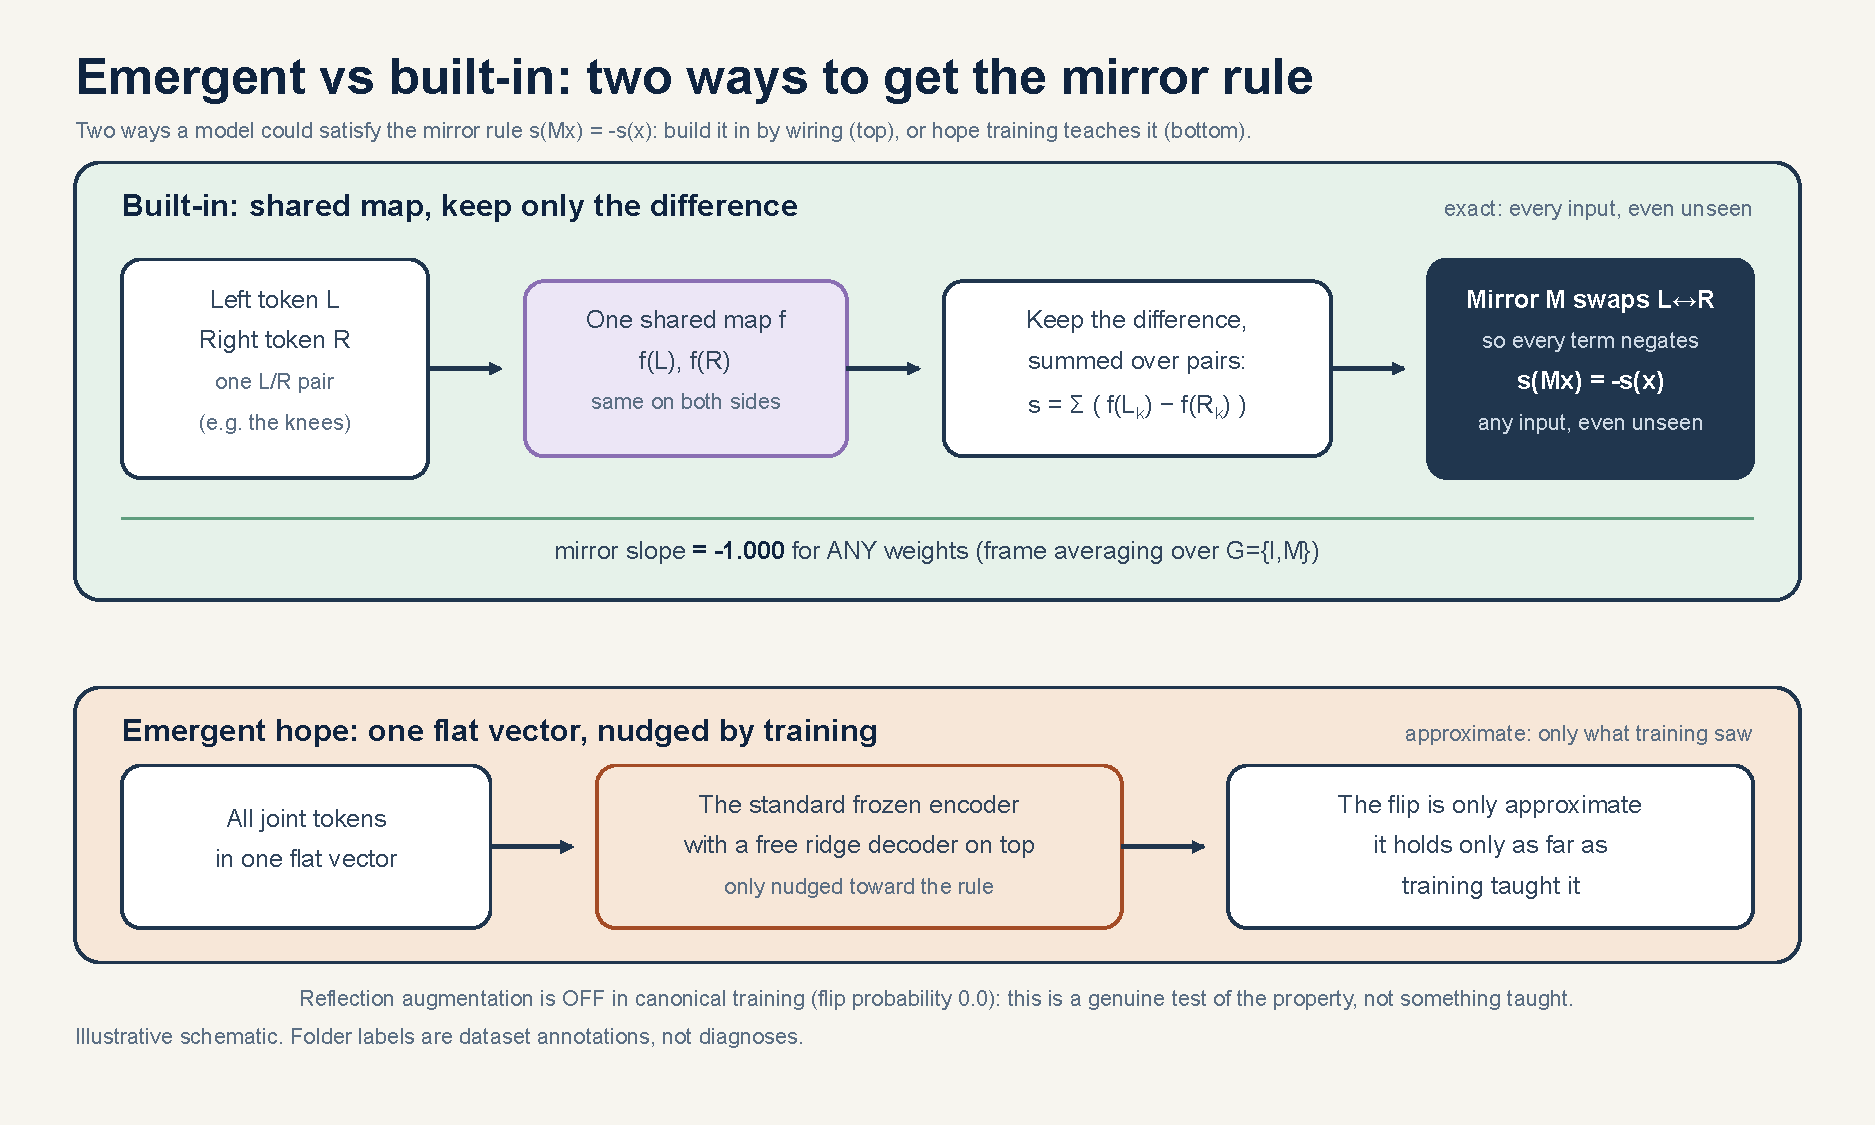
\includegraphics[width=0.62\linewidth]{fig4_construction.pdf}
  \caption{Frame averaging over $\{I,M\}$. The antisymmetric part $\Phi=A(x)-A(Mx)$ has decoded mirror slope exactly $-1$ for any nonzero weights; the symmetric part $\Psi=A(x)+A(Mx)$ has slope $+1$ and cannot predict an antisymmetric target.}
  \label{fig:construction}
\end{figure}

\begin{table}[t]
  \centering
  \caption{E2 read-out (626 primary). A, $\Phi$ (learned), and $\Phi$ (untrained) report repeated-CV means with stability intervals; $\Psi$ is a single-partition diagnostic; mirror slopes are single-partition.}
  \label{tab:e2}
  \begin{tabular}{lrr}
    \toprule
    Read-out & $R^2$ & Mirror slope \\
    \midrule
    A --- free ridge (repeated CV)                       & 0.198 [0.175, 0.221] & $-0.703$ \\
    \textbf{$\Phi$ --- frame-averaged, learned (repeated CV)} & \textbf{0.273 [0.253, 0.294]} & \textbf{$-1.0000001$} \\
    $\Phi$ --- frame-averaged, untrained (repeated CV)   & 0.219 [0.175, 0.264] & $-0.99999996$ \\
    $\Psi$ --- symmetric part (single-partition)         & 0.015 & $+1.000$ \\
    \bottomrule
  \end{tabular}
\end{table}

Two observations stand out. \textbf{(1) Built-in beats free} in repeated-CV mean ($0.273$ vs $0.198$; disjoint stability intervals---a partition-stability heuristic, not a formal test): imposing the geometry unlocks decodable structure the free read-out does not reach from the \emph{same frozen encoder}---$\Phi$ additionally evaluates the mirrored input $A(Mx)$. \textbf{(2) The controls are consistent with the antisymmetric tie---not capacity or the extra pass---as the source of the gain, but they do not isolate a causal decomposition.} The symmetric $\Psi$ cannot predict an antisymmetric target ($0.015$, slope $+1$; single-partition); a shared-map equivariant MLP is exactly antisymmetric and scores $0.243$ (single-partition; linear $\Phi$ already optimal, nonlinearity adds nothing); an unconstrained $\ge$-capacity MLP that sees both passes but is \emph{untied} collapses to $0.047$ (single-partition) with slope $-0.430$. Decomposing the point estimates, $\Phi$ exceeds free $A$ by $0.075$ in repeated-CV mean; the corresponding architecture and learned-encoder contrasts ($\Phi_\text{floor}-A$ and $\Phi-\Phi_\text{floor}$) are $0.021$ and $0.054$, with overlapping intervals---so the \emph{learning} benefit is suggestive, not decisive. $\Phi$ remains far below the raw ceiling (sign consistency $0.568$); the constructed read-out is exactly antisymmetric but explains only part of the target variance on the audited cohort, motivating pushing symmetry into the encoder.

\section{E3 --- reflection-equivariant encoder}\label{sec:e3}

\subsection{Frame-averaged encoder (zero-retrain, exact)}

Averaging the \emph{encoder} rather than the read-out, $E'(x)[t,j]=\tfrac12\big(E(x)[t,j]+E(Mx)[t,\sigma(j)]\big)$ with $\sigma$ the left/right joint permutation, makes the frozen encoder \textbf{exactly token-level reflection-equivariant with no retraining}: token-equivariance error, diff-block antisymmetry error, and sum-block symmetry error are all $0.0$ to machine precision. The laterality feature on $E'$ splits exactly into an antisymmetric $\ell-r$ block (slope $-1$ for any nonzero read-out; $R^2=0.253$ $[0.226,0.280]$) and a symmetric $\ell+r$ block. This antisymmetric block \emph{corresponds to} E2's $\Phi$ and realizes the same exact slope-$-1$ guarantee, but is not numerically identical: it equals (up to per-fold standardization) one half of $\Phi$'s $\ell-r$ sub-block, whereas $\Phi$ additionally antisymmetrizes the $\ell+r$ block---nonzero only because the original encoder is not itself equivariant---which is why $\Phi$ scores slightly higher ($0.273$ vs $0.253$; overlapping stability intervals). Honest boundary: a \emph{free} ridge on the full $E'$ feature still gives slope $-0.767$---encoder equivariance does not force an antisymmetric \emph{decoder}.

\subsection{Does reflection augmentation induce it? (a single-seed negative)}\label{sec:e32}

We retrain Stage-0 (the \texttt{normal}-annotated rows only, 270 sequences / 29 sources, 300 epochs) with one switch: sample-level consistent reflection augmentation on ($p=0.5$) vs off ($0.0$), identical trainer, seed, and hardware \citep{benton2020augerino}. Augmentation changes the objective (final JEPA loss $0.807$ vs $0.720$) but not the geometry (Table~\ref{tab:e32}). The negative rests on the mirror \emph{slope}, not on decodability: the augmented and untrained axes have similar repeated-CV means ($0.062$ $[0.011,0.114]$ vs $0.078$ $[0.013,0.144]$; overlapping stability intervals), and the free-readout slope does not move toward $-1$. Strikingly, the \textbf{untrained} encoder has the slope \emph{closest} to $-1$ ($-0.818$, vs the augmented arm's $-0.510$, the \emph{furthest})---so in this single-seed arm slope proximity alone is not evidence of learned equivariance (it is consistent with sensitivity to feature geometry), which is precisely why the by-construction guarantee (exact $-1$ for any nonzero weights) is the right instrument. This arm is a single-seed proof-of-concept, so we report it as a single-seed negative rather than a population claim.

\begin{table}[t]
  \centering
  \caption{E3.2 augmentation ablation (270 \texttt{normal}-annotated rows, transductive). A\_free reports repeated-CV means with stability intervals; free-readout slopes are single-partition.}
  \label{tab:e32}
  \begin{tabular}{lrr}
    \toprule
    Encoder & A\_free $R^2$ (stability interval) & Free-readout slope \\
    \midrule
    arm\_on (flip 0.5)      & $+0.062$ [$+0.011$, $+0.114$] & $-0.510$ \\
    arm\_off (flip 0.0)     & $-0.049$ [$-0.113$, $+0.016$] & $-0.753$ \\
    canonical Stage-0       & $-0.022$ [$-0.075$, $+0.031$] & $-0.553$ \\
    \textbf{untrained floor}& \textbf{$+0.078$ [$+0.013$, $+0.144$]} & \textbf{$-0.818$} \\
    \bottomrule
  \end{tabular}
\end{table}

\section{Discussion: the emergent-vs-built-in ladder}

The four experiments form a $2\times2$ grid (Fig.~\ref{fig:ladder}): symmetry in the \emph{read-out} or the \emph{encoder}, \emph{hoped for} or \emph{built in}. Emergent read-out (E1): slope $-0.70$, learned $\approx$ floor, gates fail; built-in read-out (E2): slope $-1.0000$, $0.273>0.198$ (disjoint intervals). Emergent encoder (E3.2): slope not toward $-1$, axis $\le$ floor; built-in encoder (E3.1): token error $0.0$, exact block split.

\begin{figure}[t]
  \centering
  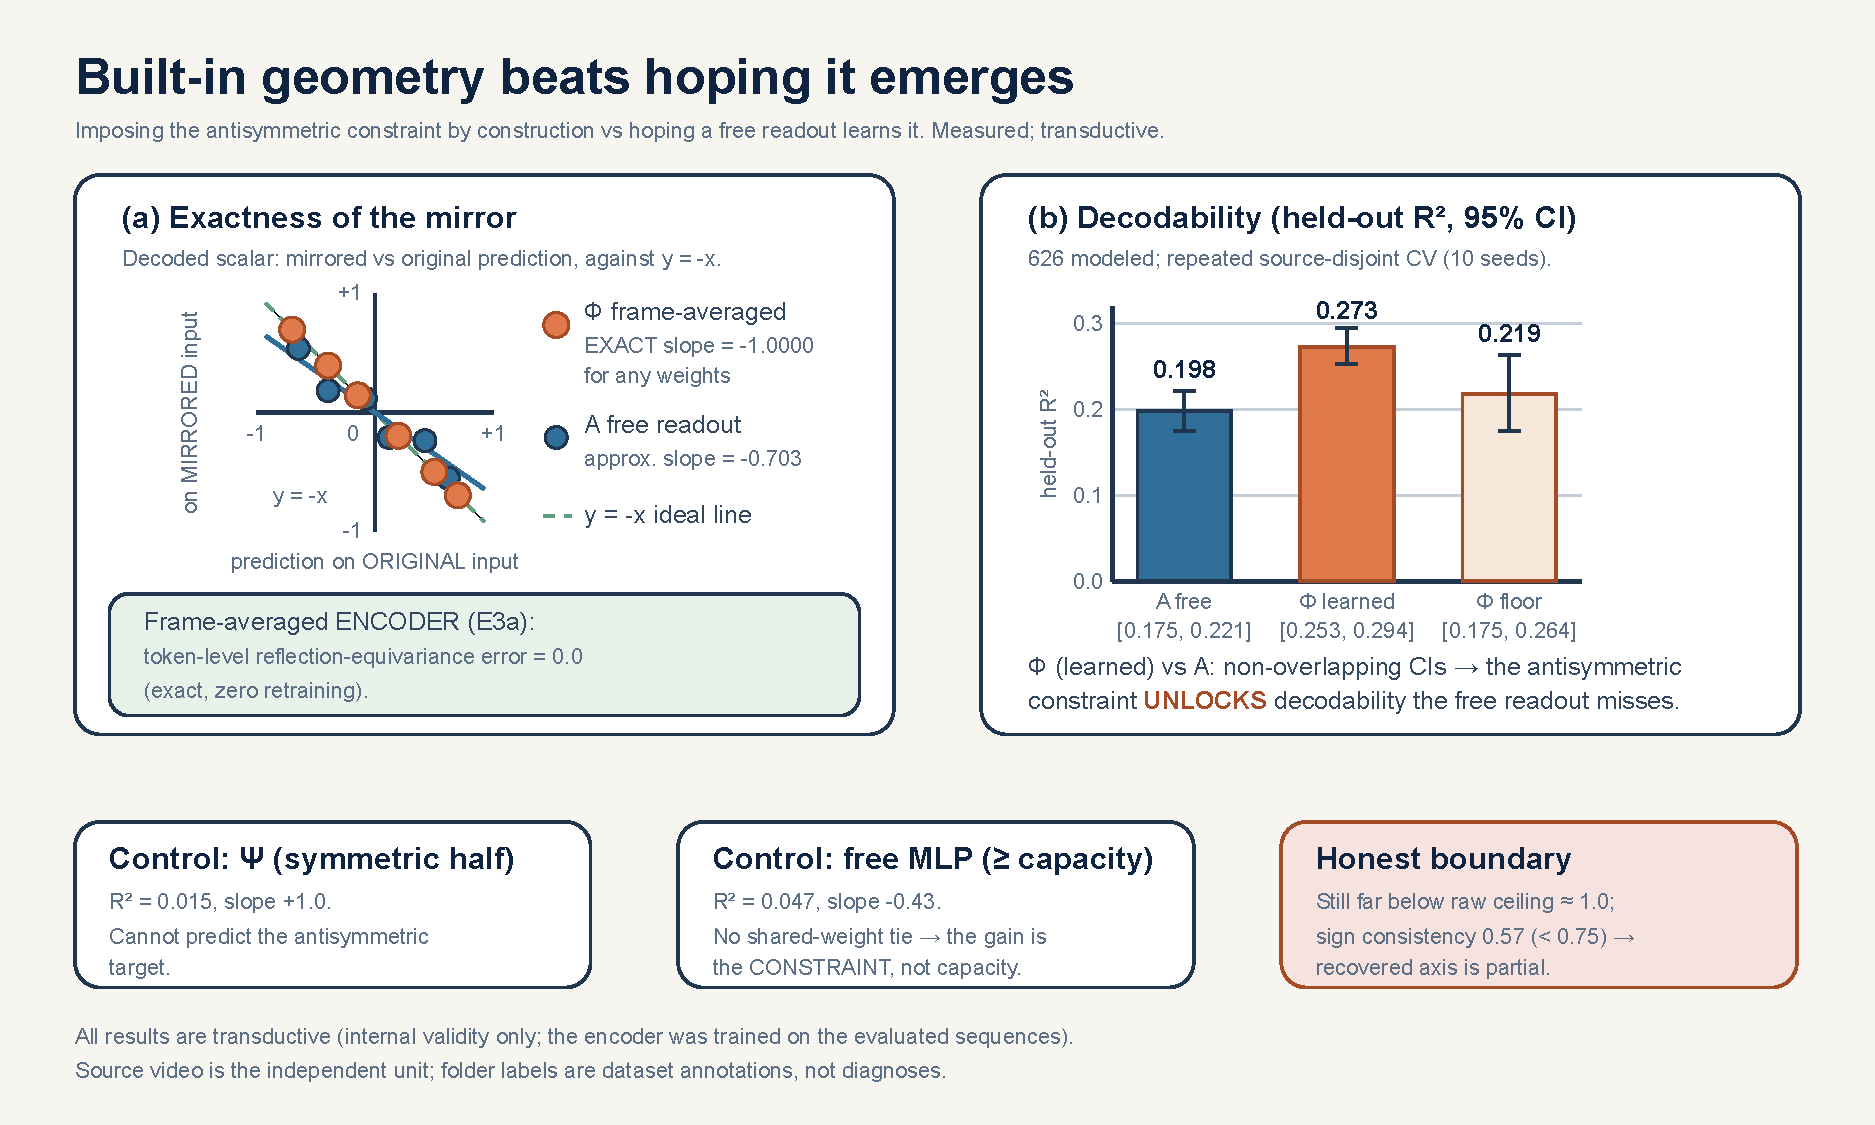
\includegraphics[width=0.68\linewidth]{fig5_builtin_beats_emergent.pdf}
  \caption{Built-in beats emergent. Left: the emergent read-out (E1) sits at or below floor with mirror slope $-0.70$; the frame-averaged read-out (E2) reaches $0.273$ with slope exactly $-1$. Right: the same contrast at the encoder---augmentation (E3.2) does not induce the axis, while the frame-averaged encoder (E3.1) is exactly equivariant.}
  \label{fig:builtin}
\end{figure}

\begin{figure}[t]
  \centering
  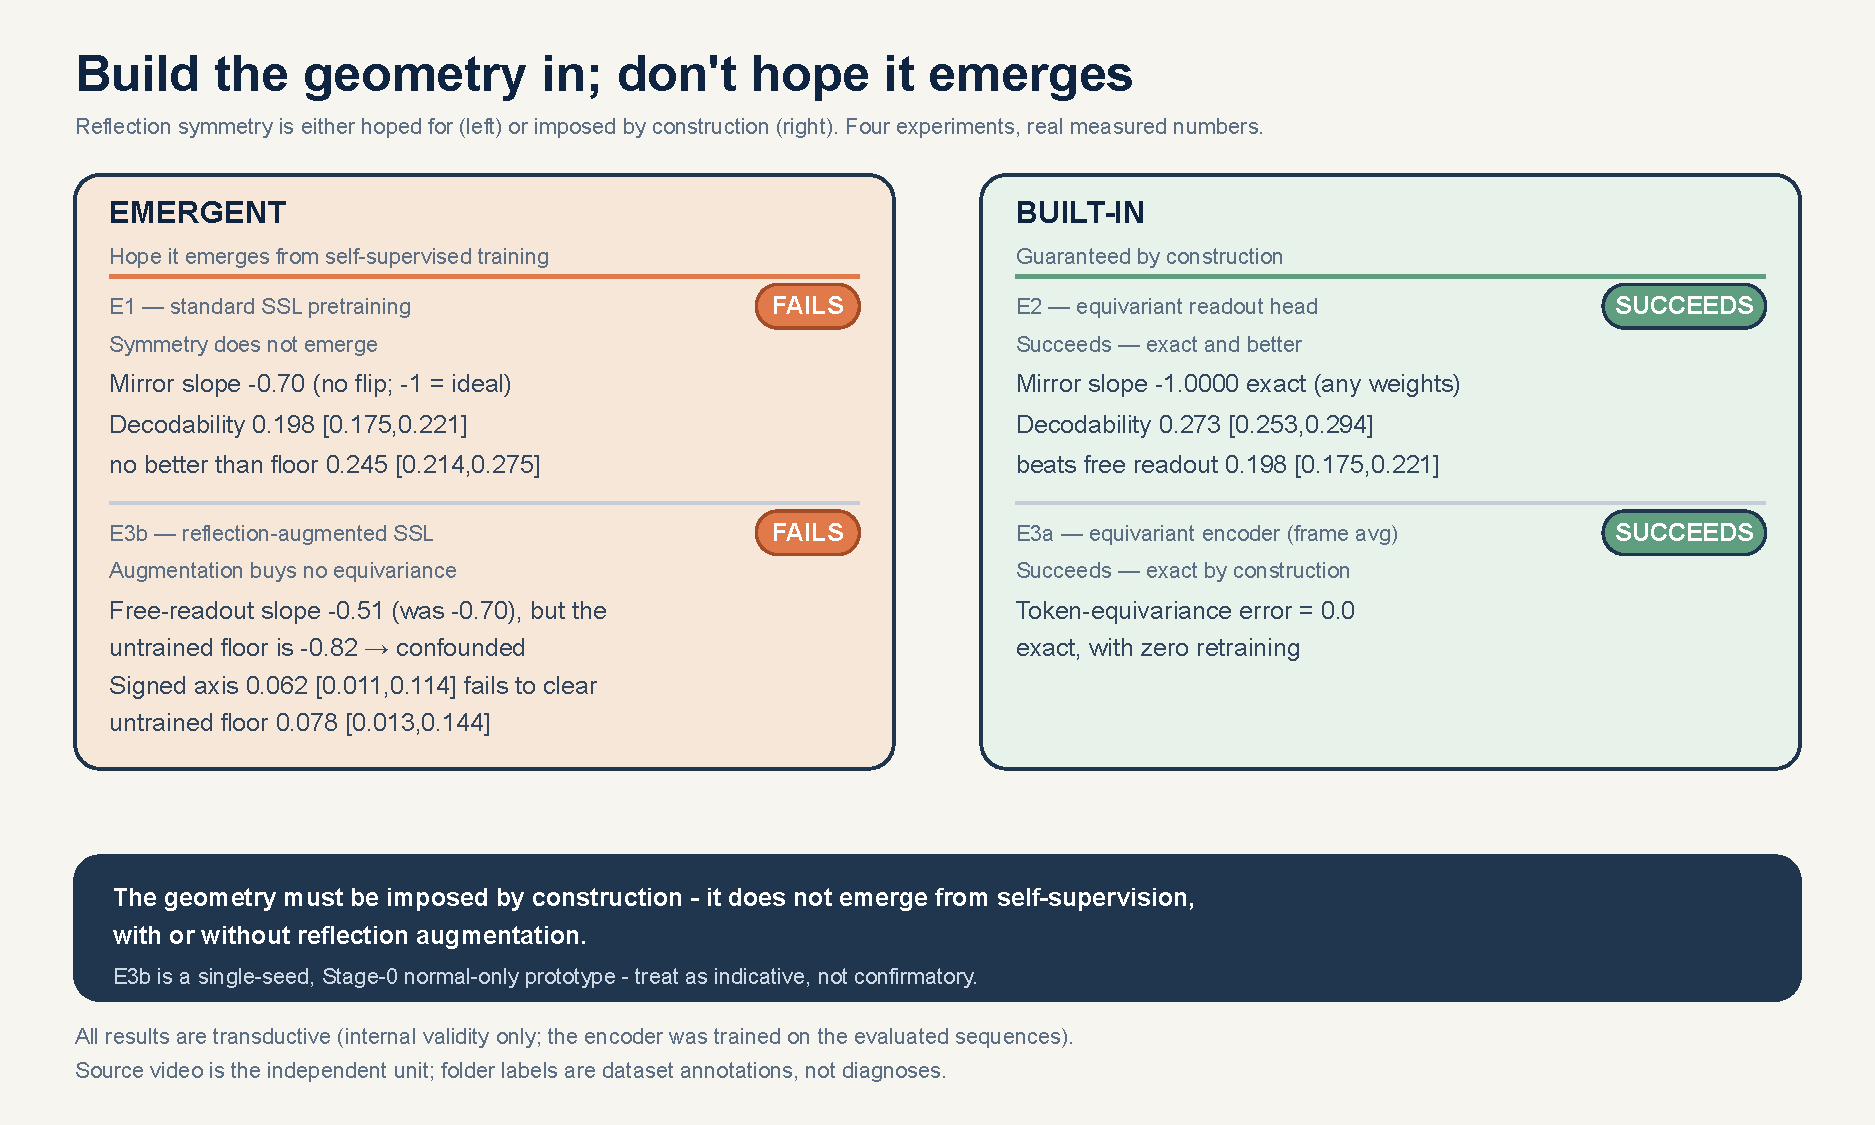
\includegraphics[width=0.66\linewidth]{fig6_ladder.pdf}
  \caption{The design ladder for geometry-aware world models: hoping symmetry emerges (E1, E3.2) fails or is unreliable on the audited system; imposing it by frame averaging (E2, E3.1) makes it exact and cheap. \emph{Build the geometry in; don't hope it emerges.}}
  \label{fig:ladder}
\end{figure}

Every row tells the same story (Fig.~\ref{fig:builtin}): in the audited system---this frozen curriculum checkpoint, and a single-seed reflection-augmentation arm---standard and reflection-augmented self-supervision leave bilateral symmetry un-learned, while frame averaging the read-out or encoder recovers it to machine precision with zero or minimal retraining. The constructive half of this finding is general (frame averaging imposes exact $\mathbb{Z}/2$ equivariance by construction); the negative half is scoped to what we audited. For geometry-aware world models of articulated bodies, the practical reading is that symmetry is cheap to \emph{impose} and---at least here---not reliably obtained by \emph{hoping} it emerges.

\section{Limitations}

Results are \textbf{transductive}---the encoder was trained on the evaluated sequences---so they carry internal validity only and do not speak to generalization to new sources; fold-local full retraining would be required for that. The signed target captures one scalar ($\mathbb{Z}/2$) symmetry, not the full kinematic tree; the augmentation arm is a single-seed prototype on the \texttt{normal}-annotated rows. The recovered axis, even built-in, remains well below the raw ceiling; the constructed read-out is exactly antisymmetric but explains only part of the target variance on the audited cohort. The curriculum's later stages are label-informed, so ``the world model'' is not purely self-supervised across all stages.

\section{Ethics and data-use}

We study a public gait dataset (GAVD \citep{ranjan2025gavd, gavdRepo2026}) whose official distribution provides annotations and public YouTube video URLs rather than raw video files; users retrieve media independently and are responsible for YouTube's terms of service, institutional ethics review, and applicable copyright, privacy, and data-protection rules. This analysis uses derived pose sequences and does not infer identity; no raw video or identity-bearing frames are redistributed. \textbf{The workspace does not currently contain a recorded institutional ethics determination or completed data-use review; both must be resolved before submission.} The dataset's condition folders (\texttt{normal}, \texttt{parkinsons}, \texttt{stroke}, \texttt{myopathic}, \texttt{cerebralpalsy}) are \textbf{dataset annotations, not diagnoses}; the independent unit of analysis is the source video, not the individual, and no clinical claim is made or implied.

\section{Conclusion}

Bilateral symmetry is a natural geometry audit for skeleton world models. The audited S-JEPA fails it---for this checkpoint, bilateral symmetry does not emerge as a decodable, sign-flipping axis, and a single-seed reflection-augmentation arm does not induce it---but frame averaging recovers the axis by construction, exactly, at the read-out or the encoder. The constructive principle generalizes even where the negative is scoped to what we tested: for physical-world models of articulated bodies, \emph{build the geometry in; don't hope it emerges.}

\begin{ack}
Anonymized for double-blind review.
\end{ack}

{\small
\bibliographystyle{plainnat}
\bibliography{../references}
}

\end{document}
